%----------------------------------------------------------------------------------------
%	PACKAGES AND THEMES
%----------------------------------------------------------------------------------------
\documentclass[aspectratio=169,xcolor=dvipsnames]{beamer}
\usetheme{Simple}

\usepackage{hyperref}
\usepackage{booktabs} % Allows the use of \toprule, \midrule and \bottomrule in tables
\usepackage{multicol}
 \usepackage{array,multirow,graphicx}
\usepackage{tikz}
\usetikzlibrary{positioning}
\usepackage{multimedia}
\usepackage[numbers]{natbib}

%----------------------------------------------------------------------------------------
%	TITLE PAGE
%----------------------------------------------------------------------------------------

% The title
\title[EECS 753 Project]{Curvy DeepPicar}
\subtitle{Using B\`ezier Curves Scheduling Steering Control}

\author[McNamee] {Patrick McNamee}
\institute[KU] % Your institution may be shorthand to save space
{
    % Your institution for the title page
    Department of Computer Science and Electrical Engineering \\
    University of Kansas
    \vskip 3pt
}
\date{\today} % Date, can be changed to a custom date


%----------------------------------------------------------------------------------------
%	PRESENTATION SLIDES
%----------------------------------------------------------------------------------------

\begin{document}

\begin{frame}
    % Print the title page as the first slide
    \titlepage
\end{frame}

\begin{frame}{Previous Work}
    \begin{multicols}{2}
    {\hfill \Large\bfseries DeepPicar \hfill}
    \begin{figure}[hbt!]
        \centering
        \includegraphics[width=1.5in]{../figures/presentation/DeepPicar.jpg}
        \caption{DeepPicar Vehicle \cite{bechtel2018picar}}
        \label{fig:deeppicar-vehicle}
    \end{figure}
    
    
    \columnbreak
    
    {\hfill \Large\bfseries DeepRacing \hfill}
    \begin{figure}[hbt!]
        \centering
        \includegraphics[width=2.5in]{../figures/presentation/deepracing-controls.PNG}
        \caption{Overview of CNN control schemes \cite{deepracing}}
        \label{fig:dr-controls}
    \end{figure}
    \end{multicols}
\end{frame}

\begin{frame}{B\`ezier Loss Function}
    
    $$ \mathbf{B}(t) = \sum_{k=0}^n \genfrac(){0pt}{0}{n}{k} (1-t)^{n-k}t^k \mathbf{P}_k \quad t\in [0, 1] $$
    Matrix Form from \cite{deepracing}: $\mathbf{B}(\mathbf{t}) = \mathbf{A}(\mathbf{t}, n)\mathbf{P}$
    
    \begin{multicols}{2}
    
    \begin{center}
        Model Output
    
        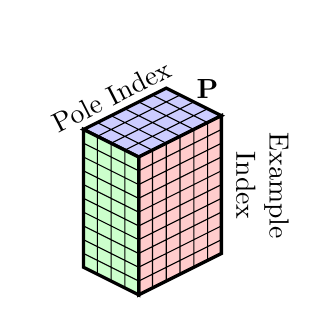
\begin{tikzpicture}[scale=0.175,every node/.style={minimum size=1cm},on grid]
        % Top
        \begin{scope}[
            yshift=-83,every node/.append style={
            yslant=0.5,xslant=-1},yslant=0.5,xslant=-1
            ]
            \filldraw[fill=blue!20] (0,0) rectangle (6, 4);
            \draw[step=1, black] (0,0) grid (6,4); %defining grids
            \draw[black,very thick] (0,0) rectangle (6,4);%marking borders
        \end{scope}
        \begin{scope}[
            yshift=-83,every node/.append style={
            yslant=0,xslant=0},yslant=0.5,xslant=0
            ]
            \filldraw[fill=red!20] (0,0) rectangle (6, -10);
            \draw[step=1, black] (0,0) grid (6,-10); %defining grids
            \draw[black,very thick] (0,0) rectangle (6,-10);%marking borders
        \end{scope}
        \begin{scope}[
            yshift=-83,every node/.append style={
            yslant=0,xslant=0},yslant=-0.5,xslant=0
            ]
            \filldraw[fill=green!20] (0,0) rectangle (-4, -10);
            \draw[step=1, black] (0,0) grid (-4,-10); %defining grids
            \draw[black,very thick] (0,0) rectangle (-4,-10);%marking borders
        \end{scope}
        
        \draw (-2,1.5) node[rotate=27] {Pole Index};
        \node at (5,2) {$\mathbf{P}$};
        \draw (9,-5) node[rotate=-90, align=center] {Example\\ Index};
        \end{tikzpicture}
    \end{center}
    
    \columnbreak
    
    \begin{center}
        Actual Output
        
        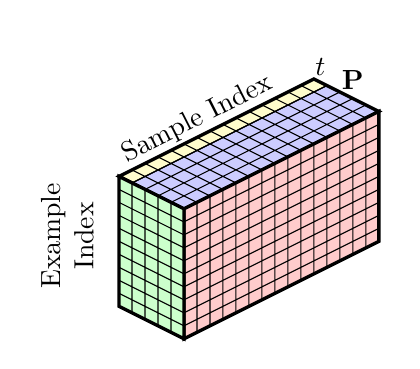
\begin{tikzpicture}[scale=0.165,every node/.style={minimum size=1cm},on grid]
        % Top
        \begin{scope}[
            yshift=-83,every node/.append style={
            yslant=0.5,xslant=-1},yslant=0.5,xslant=-1
            ]
            \filldraw[fill=blue!20] (0,0) rectangle (15, 4);
            \filldraw[fill=yellow!20] (0,4) rectangle (15, 5);
            \draw[step=1, black] (0,0) grid (15,5); %defining grids
            \draw[black,very thick] (0,0) rectangle (15,5);%marking borders
        \end{scope}
        \begin{scope}[
            yshift=-83,every node/.append style={
            yslant=0,xslant=0},yslant=0.5,xslant=0
            ]
            \filldraw[fill=red!20] (0,0) rectangle (15, -10);
            \draw[step=1, black] (0,0) grid (15,-10); %defining grids
            \draw[black,very thick] (0,0) rectangle (15,-10);%marking borders
        \end{scope}
        \begin{scope}[
            yshift=-83,every node/.append style={
            yslant=0,xslant=0},yslant=-0.5,xslant=0
            ]
            \filldraw[fill=green!20] (0,0) rectangle (-5, -10);
            \draw[step=1, black] (0,0) grid (-5,-10); %defining grids
            \draw[black,very thick] (0,0) rectangle (-5,-10);%marking borders
        \end{scope}
        
        \draw (1,4) node[rotate=27] {Sample Index};
        \draw (-9,-5) node[rotate=90, align=center] {Example\\ Index};
        \draw (10.5,8) node {$t$};
        \draw (13,7) node {$\mathbf{P}$};
        \end{tikzpicture}
    \end{center}
    
    \end{multicols}
    
\end{frame}

\begin{frame}{DeepPicar Dataset}
    
    
    Image and point pair at every 0.05 seconds/50 milliseconds/20Hz and labeled incorrectly as microseconds in data. Using a moving average filter to approximate continuous control inputs.

\begin{multicols}{2}


\begin{table}[hbt]
    \centering
    \caption{Output Data from Video 1}
    \resizebox{!}{0.75in}{
    \begin{tabular}{r|c|l}
        Time [ms] & Frame & Wheel Angle [rad]\\\hline\hline
        1527606810546&	30&	0\\
        1527606810596&	31&	0\\
        1527606810646&	32&	0\\
        1527606810696&	33&	0\\
        1527606810746&	34&	0\\
        1527606810796&	35&	0.523598776\\
        1527606810846&	36&	0.523598776\\
        1527606810896&	37&	0.523598776\\
        1527606810946&	38&	0.523598776\\
        1527606810996&	39&	0.523598776\\
        1527606811046&	40&	0.523598776\\
        1527606811096&	41&	0.523598776\\
        1527606811146&	42&	0\\
        1527606811196&	43&	0\\
        1527606811246&	44&	0\\
        1527606811296&	45&	0\\
        1527606811346&	46&	0\\
        1527606811396&	47&	0\\
    \end{tabular}}
    \label{tab:data}
\end{table}

\columnbreak

\begin{figure}[hbt]
    \centering
    \includegraphics[width=2.25in]{../figures/presentation/out-video-1-moment.jpg}
    \caption{Example Image from Video 1\cite{bechtel2018picar}}
    \label{fig:input-image}
\end{figure}

\end{multicols}    
\end{frame}

\begin{frame}{Training the Networks}
    \begin{itemize}
        \item Train on 9 of 11 videos.
        \item Train on only 200 of 1000 images of a video at once. Horizontally flip the image as well.
        \item 80-20 Test Validation split.
        \item Train 50 epochs every 200 frames and loop over videos a total of 4 times.
        \item B\`ezier CNN is 2 Hz controller over 0.2 seconds with 3rd degree polynomial.
    \end{itemize}

\begin{multicols}{2}

\begin{figure}[hbt]
    \centering
    \includegraphics[height=1.25in, trim= 0in 0.25in 0in 0.0in, clip]{../figures/presentation/cnn-training-history.PNG}
    \caption{DAVE-2 CNN Training History}
    \label{fig:cnn-th}
\end{figure}

\columnbreak

\begin{figure}[hbt]
    \centering
    \includegraphics[height=1.25in, trim= 0in 0.25in 0in 0.0in, clip]{../figures/presentation/bezier-training-history.PNG}
    \caption{B\`ezier CNN Training History}
    \label{fig:bcnn-th}
\end{figure}

\end{multicols}    

\end{frame}

\begin{frame}{Accuracy Results}
    \begin{multicols}{2}
    
    \begin{table}[h]
        \centering
            \caption{Image-to-Point CNN Model (Acc: 20.45\%)}
            \begin{tabular}{|c|r|c|c|c|}
            \multicolumn{2}{c}{} & \multicolumn{3}{c}{Model Predicted}\\\cline{3-5}
            \multicolumn{1}{c}{} & & Left & Center & Right\\\hline
             \parbox[t]{2mm}{\multirow{3}{*}{\rotatebox[origin=c]{90}{Record}}} & Left & 48 & 31 & 21 \\\cline{3-5}
            & Center & 156 & 156 & 188 \\\cline{3-5}
            & Right & 54 & 136 & 205 \\\cline{3-5}\hline
            \end{tabular}
        \label{tab:i2p-acc}
    \end{table}
    
    Results based on 2 unseen test files (2000 images total). Note not there is a bias in the dataset for right turns and just going straight is correct 50\% of the time.
    
    \columnbreak
    \begin{table}[h]
        \centering
            \caption{Image-to-Point B\`ezier Model (Acc: 66.75\%)}
            \begin{tabular}{|c|r|c|c|c|}
            \multicolumn{2}{c}{} & \multicolumn{3}{c}{Model Predicted}\\\cline{3-5}
            \multicolumn{1}{c}{} & & Left & Center & Right\\\hline
             \parbox[t]{2mm}{\multirow{3}{*}{\rotatebox[origin=c]{90}{Record}}} & Left & 60 & 111 & 9 \\\cline{3-5}
            & Center & 48 & 667 & 261 \\\cline{3-5}
            & Right & 13 & 223 & 608 \\\cline{3-5}\hline
            \end{tabular}
        \label{tab:i2bp-acc}
    \end{table}
    
    \begin{table}[h]
        \centering
            \caption{Image-to-Curve B\`ezier Model (Acc; 38.10\%) }
            \begin{tabular}{|c|r|c|c|c|}
            \multicolumn{2}{c}{} & \multicolumn{3}{c}{Model Predicted}\\\cline{3-5}
            \multicolumn{1}{c}{} & & Left & Center & Right\\\hline
             \parbox[t]{2mm}{\multirow{3}{*}{\rotatebox[origin=c]{90}{Record}}} & Left & 83 & 46 & 33 \\\cline{3-5}
            & Center & 268 & 343 & 313 \\\cline{3-5}
            & Right & 177 & 268 & 336 \\\cline{3-5}\hline
            \end{tabular}
        \label{tab:i2bc-acc}
    \end{table}
    
    \end{multicols}
\end{frame}

\begin{frame}{Overlayed Results}

    {\vfill {\hfill \Large\bfseries To the videos! \hfill} \vfill}
    
\end{frame}

\begin{frame}[allowframebreaks]{References}
    \bibliographystyle{IEEEtranN}
    \bibliography{citations}  
\end{frame}

\end{document}